%% -*- ispell-local-dictionary: "es" -*-

\documentclass[a4paper,twoside]{article}
\usepackage[utf8]{inputenc}
\usepackage[spanish]{babel}
\usepackage{indentfirst}
\usepackage{fancybox}
\usepackage{epsfig}
\usepackage{tabularx}
\usepackage{sectsty}
\usepackage{amsmath}
\usepackage{float}
\usepackage{listings}
\usepackage{color}
%\usepackage{subfigure}
\usepackage[colorlinks=true,linkcolor=blue,urlcolor=blue]{hyperref}
%\usepackage{placeins}
\usepackage{verbatim}
%\usepackage[table]{xcolor}
%\usepackage{multirow}
\usepackage{rotating}
\usepackage{pdflscape}
%\usepackage{natbib}


\newcolumntype{R}{>{\raggedleft\arraybackslash}X}
\newcolumntype{C}{>{\centering\arraybackslash}X}


\marginparwidth 0pt     \marginparsep 0pt
\topmargin   0pt        \textwidth   6.5in
\textheight 23cm
% Margen izq del txt en impares.
\setlength{\oddsidemargin}{.0001\textwidth}
% Margen izq del txt en pares.
\setlength{\evensidemargin}{-.04\textwidth}
% Anchura del texto
\setlength{\textwidth}{.99\textwidth}


\lstset{ %
  language=Java,                     % choose the language of the code
  basicstyle=\scriptsize\ttfamily,               % the size of the fonts that are used for the code
  numbers=left,                   % where to put the line-numbers
  numberstyle=\tiny,              % the size of the fonts that are used for the line-numbers
  stepnumber=5,                   % the step between two line-numbers. If it's 1 each line will be numbered
  numbersep=5pt,                  % how far the line-numbers are from the code
  backgroundcolor=\color{white},  % choose the background color. You must add \usepackage{color}
  showspaces=false,               % show spaces adding particular underscores
  showstringspaces=false,         % underline spaces within strings
  showtabs=false,                 % show tabs within strings adding particular underscores
  frame=single,	                  % adds a frame around the code
  tabsize=2,	                  % sets default tabsize to 2 spaces
  captionpos=t,                   % sets the caption-position to bottom
  breaklines=true,                % sets automatic line breaking
  breakatwhitespace=true,         % sets if automatic breaks should only happen at whitespace
  escapeinside={\%*}{*)},         % if you want to add a comment within your code
}


\def\assignedcell{\cellcolor[gray]{0.9}}
\def\rangecell{\cellcolor[gray]{0.7}}
\def\filtercell{\cellcolor[gray]{0.5}}
\def\nocell{\cellcolor[gray]{0.3}}



\author{Barros Barros, Ismael \\
  Fernández Núñez, Daniel \\
  Iglesias Fraga, David}
\date{\today}



\title{Práctica Web .NET -- Sitio web de comentarios de apuestas deportivas \\ Integración de Sistemas 2009-2010}
\pagenumbering{arabic} \pagestyle{myheadings} \markboth{Integración de Sistemas 2009-2010}{Práctica Web .NET}

\begin{document}
\maketitle
\cleardoublepage
\tableofcontents
%\cleardoublepage
\newpage

\section{Arquitectura global}

\begin{figure}[H]
  \centering
  \caption{Diagrama de arquitectura}
  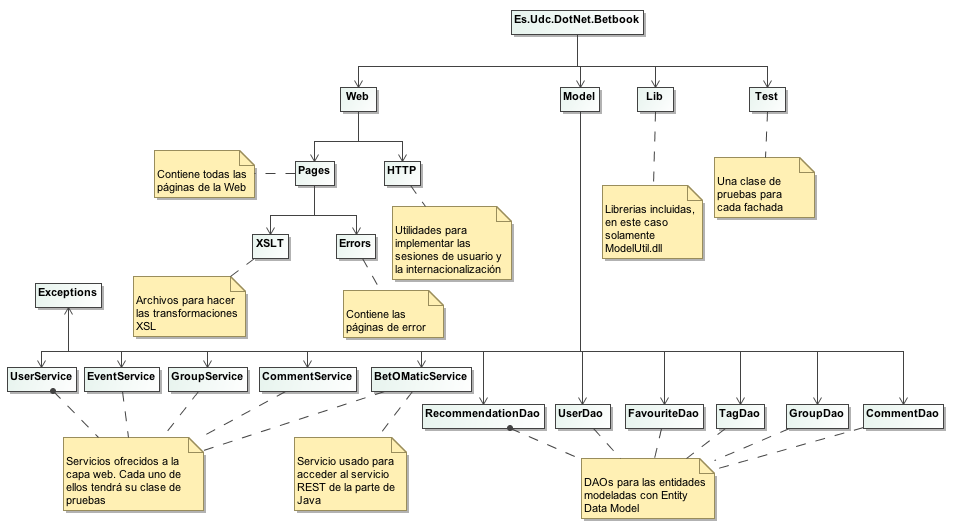
\includegraphics[width=\textheight,angle=90]{img/Arquitectura.png}
\end{figure}


\section{Modelo}


\subsection{Clases persistentes}

\begin{figure}[H]
  \centering
  \caption{Diagrama de clases persistentes}
  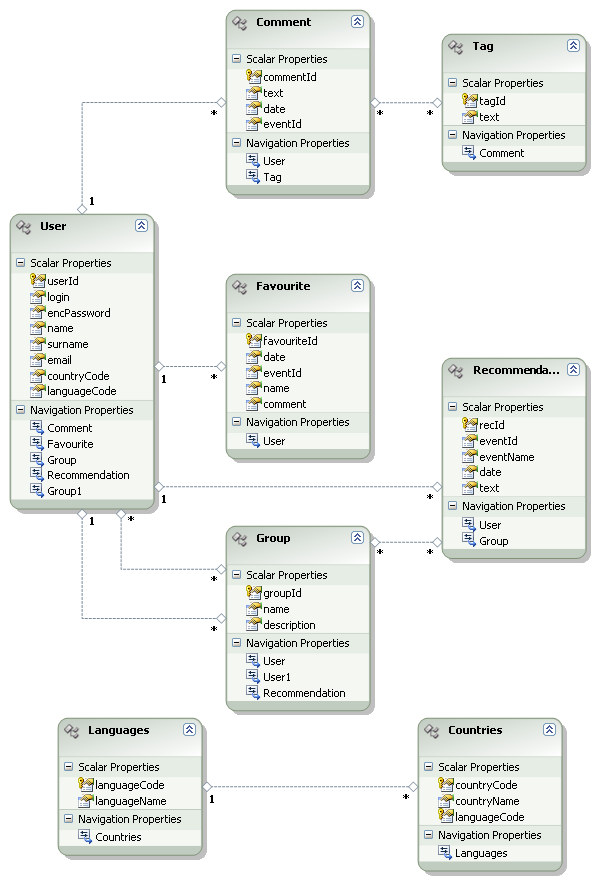
\includegraphics[height=.9\textheight]{img/Clases_persistentes.png}
\end{figure}

\newpage
\subsection{Interfaces de los servicios ofrecidos por el modelo}

\begin{figure}[H]
  \centering
  \caption{Interfaces de los servicios}
  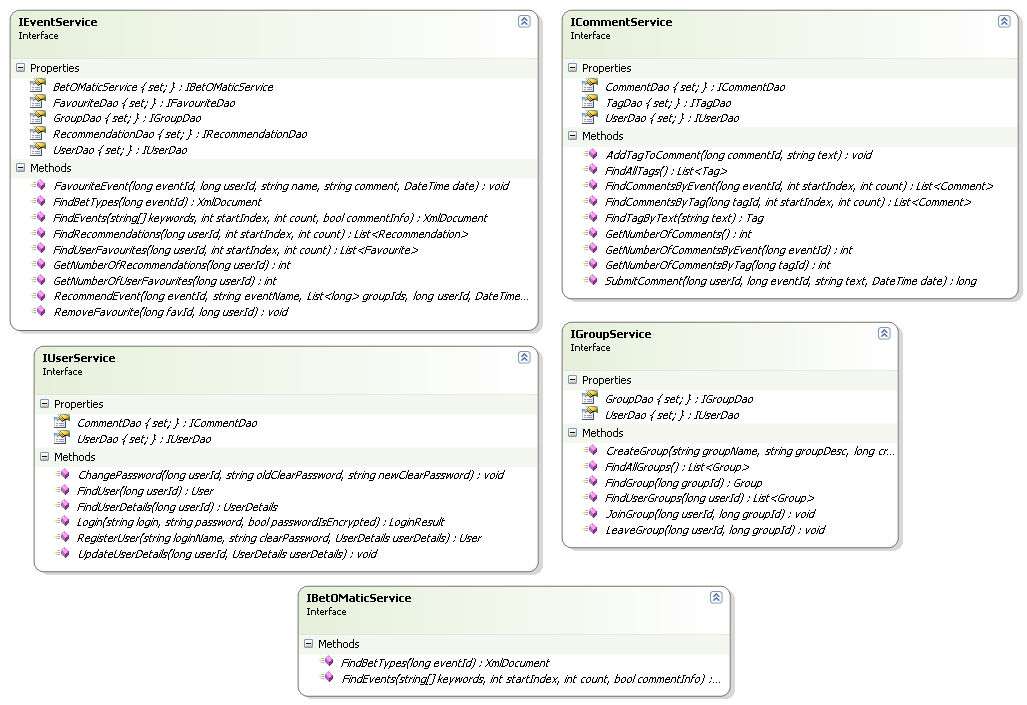
\includegraphics[width=1.1\textwidth]{img/UML_Service_interfaces.png}
\end{figure}

Se ha clasificado la funcionalidad del sistema en tres servicios, siguiendo un criterio semántico para su segmentación:

\begin{description}
\item[Servicio de usuario:] Contiene la funcionalidad referida a los perfiles de los {\bf usuarios} del sistema. Permite, por ejemplo, su registro, autenticatión y modificación
\item[Servicio de grupos:] Contiene la funcionalidad de gestión de {\bf grupos} de usuarios. Permite su creación, y que un usuario dado se una o deje un grupo.
\item[Servicio de comentarios:] Contiene la funcionalidad relacionada con la gestión de los comentarios y sus etiquetas. Los comentarios pueden ser creados, etiquetados, y buscados por evento o por etiqueta.
\item[Servicio de eventos:] Contiene la funcionalidad relacionada con {\bf eventos}, las {\bf recomendaciones} de los mismos y los {\bf favoritos}.
\end{description}


\subsection{Diseño de un DAO}

\begin{figure}[H]
  \centering
  \caption{Diagrama de clases del DAO de la clase User}
  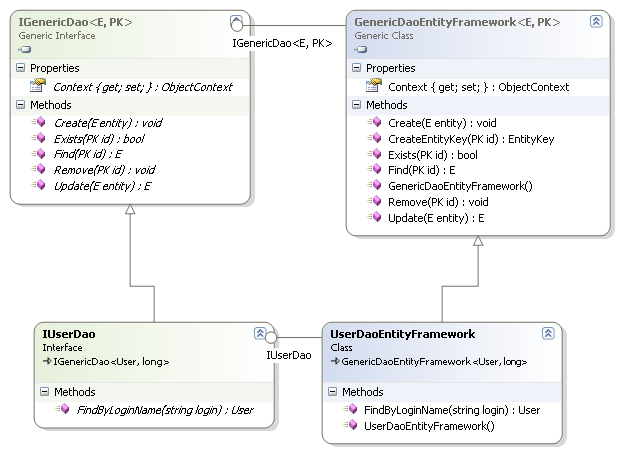
\includegraphics[width=.8\textwidth]{img/UML_DAO_implementation.png}
\end{figure}


\newpage
\subsection{Diseño de un servicio del modelo}

%% \begin{figure}[H]
%%   \centering
%%   \caption{Diagrama de clases del servicio UserService}
%%   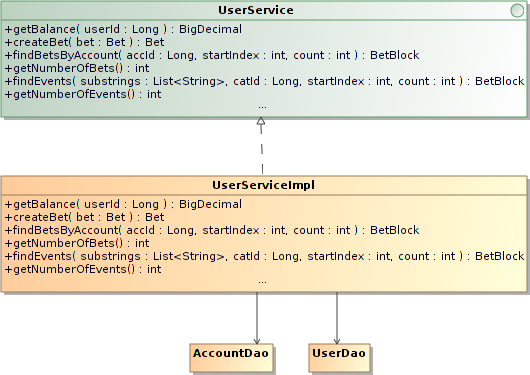
\includegraphics[width=\textwidth]{../uml/Class_Diagram__Clases_UserService.png}
%% \end{figure}

\begin{figure}[H]
  \centering
  \caption{Diagrama de clases del servicio UserService}
  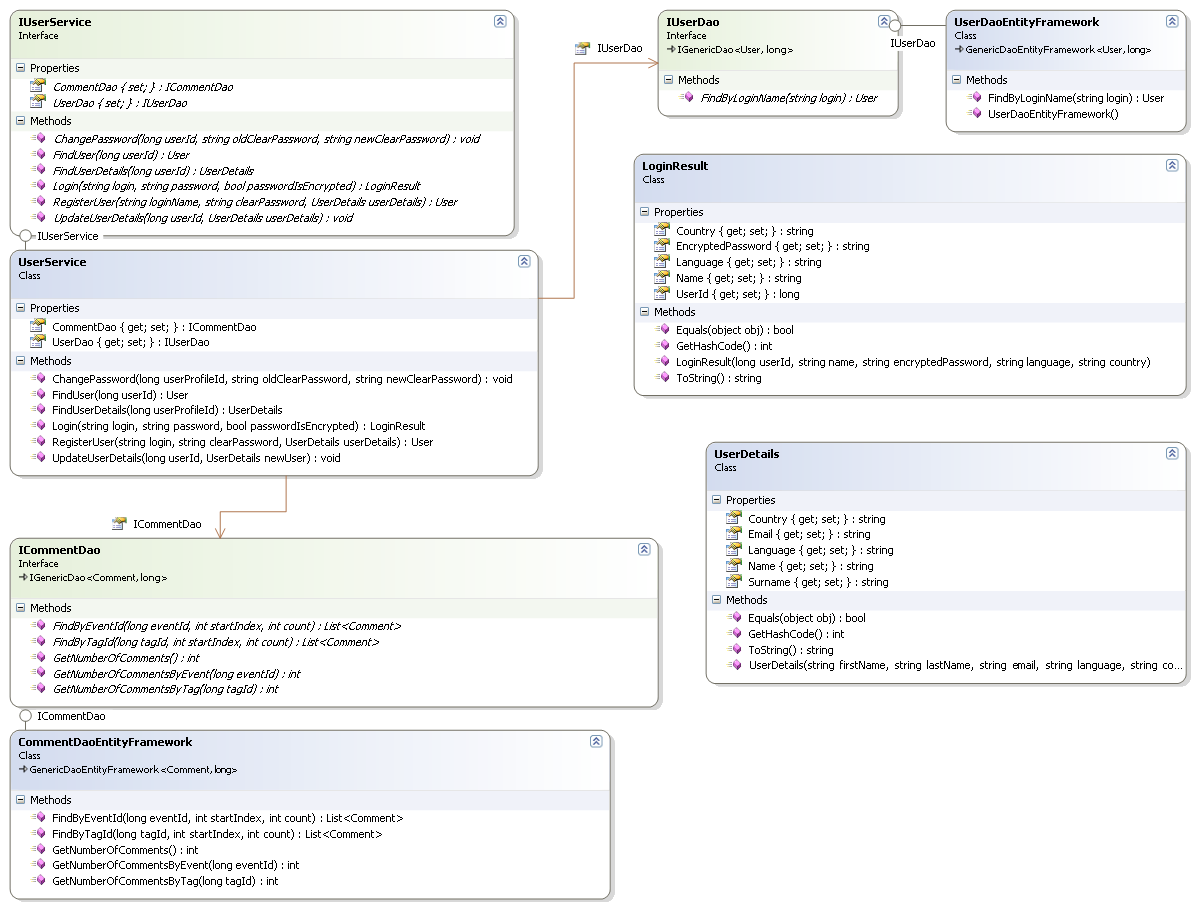
\includegraphics[width=1.1\textwidth]{img/UML_Service_implementation.png}
\end{figure}

\begin{figure}[htbp]
  \centering
  \caption{Diagrama de secuencia para el registro de usuario en el modelo}
  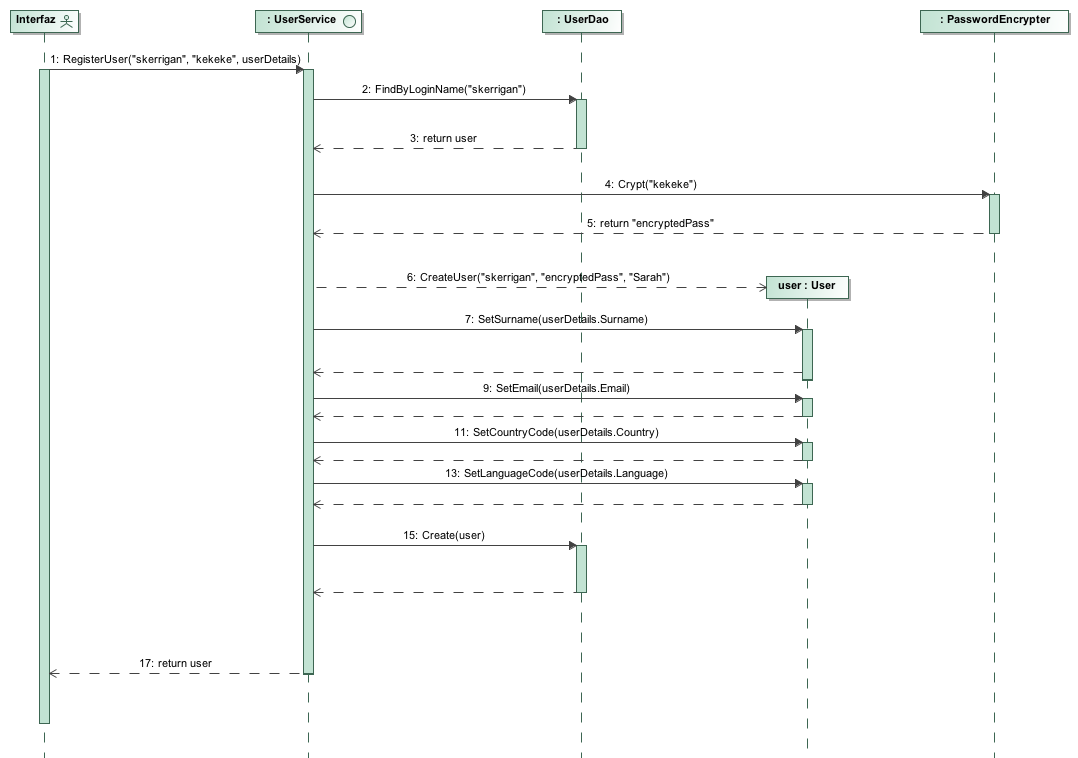
\includegraphics[width=\textheight,angle=90]{img/Secuencia_UserService.png}
\end{figure}



%\subsection{Otros aspectos}


\newpage
\section{Interfaz gráfica}

\begin{figure}[H]
  \centering
  \caption{Diagrama de secuencia del registro de un usuario en la interfaz gráfica}
  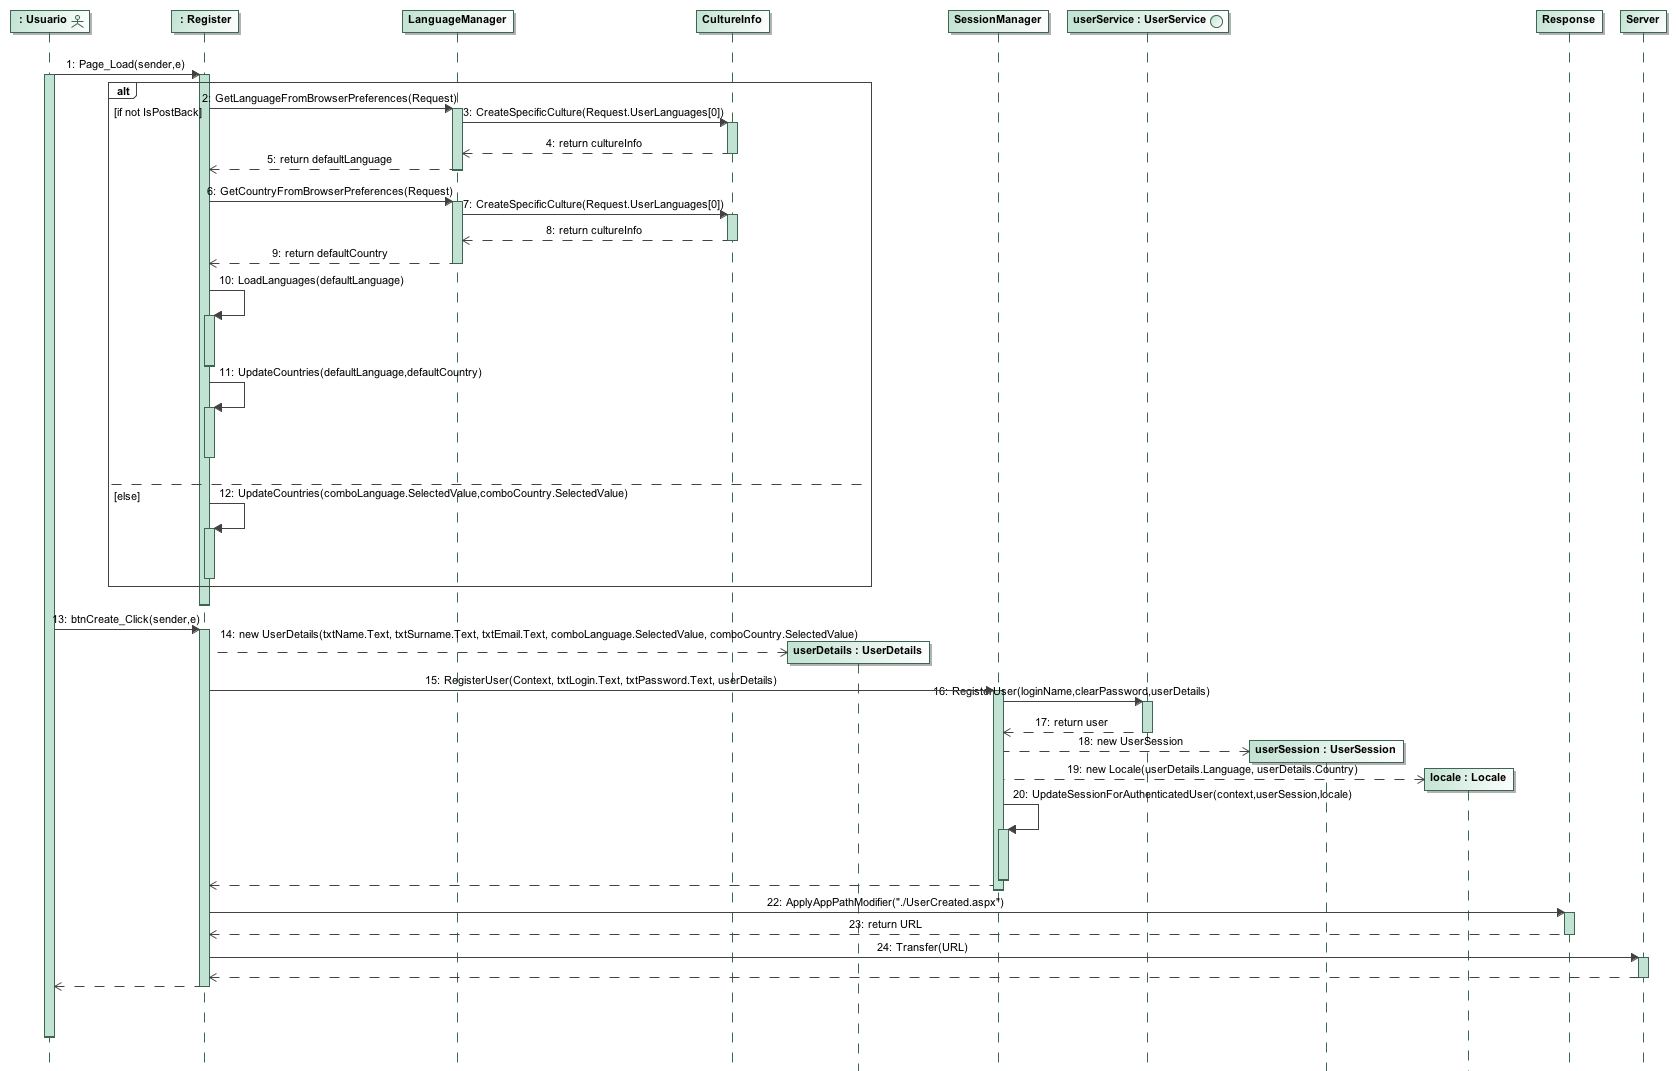
\includegraphics[width=\textheight,angle=90]{img/Sequence_Register_Web.png}
\end{figure}


\newpage
\section{Partes adicionales}

\begin{description}
\item[Parsing de XML]:

Se le permite al usuario visualizar información sobre los comentarios de cada evento en la lista de resultados del caso de uso de búsqueda de eventos.

Este caso de uso está implementado en la capa modelo obteniendo un {\it XmlDocument} a partir del servicio XML de la parte de Java de la asignatura, y devolviéndoselo intacto a la capa web para que le aplique una transformación XSLT.

Para implementar la parte opcional, la capa web le indica al modelo mediante un parámetro que el usuario requiere información de comentarios, y éste, una vez ha obtenido el {\it XmlDocument}, itera sobre cada uno de los eventos devueltos ({\tt //event}), buscando el número de comentarios existentes para cada evento e inyectándolo en el mismo {\it XmlDocument} en un nuevo elemento {\tt //event/numberOfComments}.

Una implementación alternativa habría sido crear una lista de objetos que fusionen la información de los eventos devueltos con información sobre comentarios, pero la solución propuesta se ha considerado más limpia y fácil de implementar, una vez codificada la parte obligatoria de la práctica.

\item[Etiquetado de comentarios]:

\begin{itemize}
\item Al añadir un comentario, el usuario dispone de una caja de texto adicional donde puede insertar etiquetas separadas por espacios o por comas, siguiendo un diseño similar al que siguen sitios como {\it http://www.flickr.com}. Adicionalmente, se le expone al usuario una lista con los etiquetas existentes. Cada etiqueta es un link que ejecutará una pequeña rutina escrita en Javascript, que simplemente añadirá la etiqueta a la caja de texto de etiquetas.
\item En todo momento, se expone bajo el menú principal de la aplicación una nube de etiquetas, con las etiquetas existentes en base de datos dispuestas en orden arbitrario pero con un tamaño de letra directamente proporcional al número de comentarios que fueron etiquetados con esa etiqueta.
\item Al visualizar la lista de comentarios para un evento, se muestra para cada comentario la lista de etiquetas asociadas al mismo.
\end{itemize}

En todos los casos, la lista de etiquetas se ha implementado como un simple ListView de ASP.NET, que toma como DataSource una lista de objetos {\tt Tag}. En los dos últimos casos, cada etiqueta es un link que le permite al usuario ver la lista de comentarios etiquetados con la misma.

\end{description}



\section{Compilación e instalación de la aplicación}

En un entorno con el software necesario instalado y configurado correctamente se han de seguir los siguiente pasos para compilar e instalar la aplicación:

\begin{enumerate}

\item Ejecutar el servidor de la parte Java:

\begin{enumerate}
\item {\tt \$ mysqld --defaults-file=\$HOME/.my.cnf}
\item {\tt \$ mvn jetty:run}
\end{enumerate}

\item Ejecutar la aplicación:

\begin{enumerate}
\item Botón derecho sobre el proyecto ``Web'' $>$ {\it Set as StartUp Project}
\item Botón derecho sobre ``Pages/MainPage.aspx'' $>$ {\it Set as Start Page}
\item Ejecutar el proyecto ``Web'' (Ctrl + F5)
\end{enumerate}

\end{enumerate}


\section{Problemas conocidos}

\begin{itemize}
\item La implementación de la nube de etiquetas es ineficiente, porque en cada llamada a la página, se cuenta el número de comentarios asociado a cada uno de las etiquetas, con el fin de renderizar cada etiqueta con un tamaño de letra proporcional al número de comentarios. Este detalle se podría solucionar almacenando en cada etiqueta el número de comentarios asociados al mismo, y actualizando este contador mediante triggers.
\end{itemize}


\end{document}
